\documentclass{article}
% hiermit werden alle packages in eine separate .tex datei ausgeladen
% zum Einblenden von Grafiken
\usepackage{graphicx}
% ändert die automatisch generierten wörter (inhaltsverzeichnis etc.) zu deutsch. 
% default ist englisch, also einfach das includepackage löschen.
\usepackage[german]{babel}
% um Grafiken gezielt anzuzeigen mit /begin{figure}[H] /end{figure}
\usepackage{float}
%Quelltexthighlighting, integration dessen nicht als rastergrafik, sondern skalierbar
\usepackage{minted}

\usepackage[top=2cm, bottom=2cm, outer=0cm, inner=0cm]{geometry}
\usepackage[pages=some]{background}

\begin{document}

    \tableofcontents
        test(später löschen)
    \newpage

    \listoffigures
    
    \section{Der Anfang vom Anfang.}
    Der Text ist verhext, braucht kein Slash und keine Klammern, 
    das ist der Hammer(n).
    
        Die Abbildung \ref{fig:DAVES_PANCAKES_RECIPE} zeigt das erleuterte Rezept
        in größerem Detail. 

        % line break mit leerzeichen zwischen den zeilen! so easy!
        1.) zutaten

        2.) bearbeitungsweise

        \begin{figure}[H]
            \centering
            % error 'overfull' = bild zu groß für platz, fixed indem man width auf das 0.x Fache anpasst (hier 0.5) 
            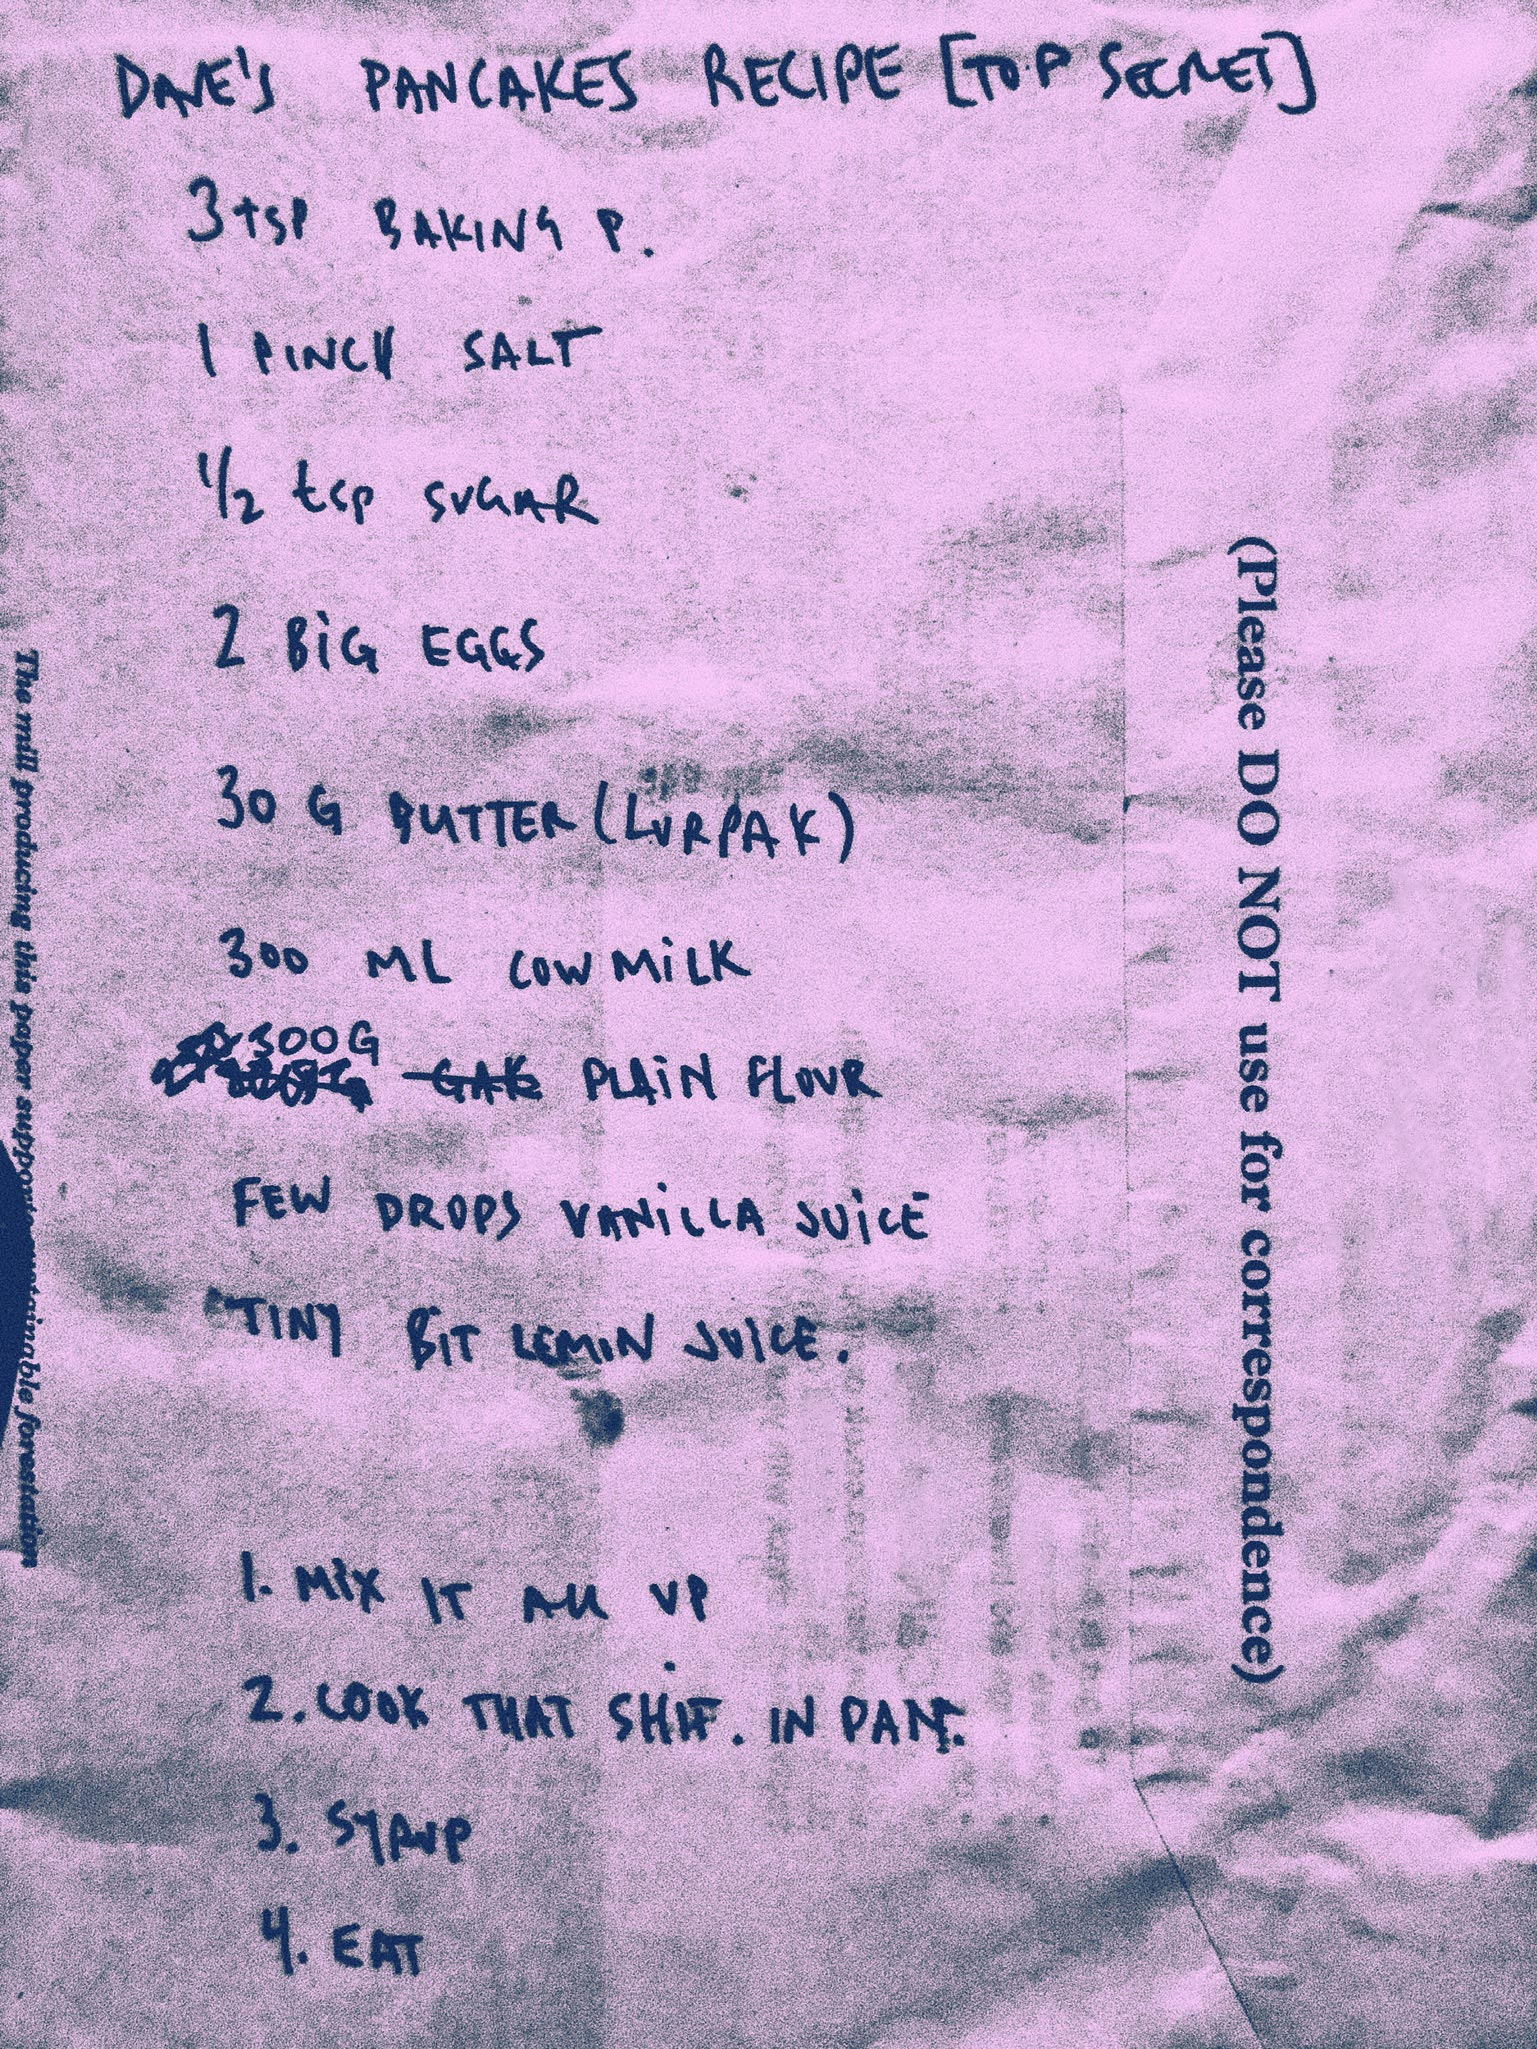
\includegraphics[width=0.5\linewidth]{graphics/DAVES_PANCAKES_RECIPE.jpg}
            \caption[cooles rezept]{Abbildung zeigt details}
    
            
            %mit label werden grafiken in texts referenziert
            \label{fig:DAVES_PANCAKES_RECIPE}
        \end{figure}
        
        \subsection {erstes Unterkapitel vom ersten Kapitel.}
        Badabing Badabum.

            \subsubsection{we need to go deeper!}

                \paragraph{insert dumb Inception joke inside the paragraph. it won't go deeper though.} 
                   
                    \subparagraph{subparagraph as smallest unit of text.}

    \section{nächstes kapitel}
    you already know. 

    
    

\end{document}




